\chapter{一些修改之处——By CYX}
2022年学校更新了双盲评审的要求与规范,同时,本人在使用祖传模版过程中,也遇到了一些问题,对前辈们的模版进行了一些细节修改,本章主要介绍本人对祖传模版的更改。

\section{双盲评审}
双盲评审论文要求隐去作者及导师信息,因此论文封面及成果列表需要进行变更,且论文构成中,盲审论文不包括致谢部分。

导言区option控制论文封面,mainManuscript.tex文末部分代码控制成果列表及致谢。
\begin{lstlisting}
    \ifpdfcover
        \ifreview
            \chapter{攻读博士学位期间取得的研究成果}

一、已发表(包括已接受待发表)的论文,以及已投稿、或已成文打算投稿、或拟成文投稿的论文情况\underline{\textbf{(只填写与学位论文内容相关的部分):}}

\begin{centering}
	\small
	\begin{longtable}{|>{\centering}m{0.5cm}|>{\centering}m{5.5cm}|>{\centering}m{2.7cm}|>{\centering}m{1.8cm}|>{\centering}m{1.8cm}|>{\centering}m{1cm}|}
		\hline 
		\textbf{序号}  & \textbf{发表或投稿刊物名称、级别}& \textbf{作者(仅注明第几作者)} & \textbf{发表年份} & \textbf{与学位论文哪一部分(章、节)相关} & \textbf{被索引收录情况}\tabularnewline
		\hline 
		1   & Journal of Manufacturing Processes\\(IF:5.01, JCR Q2) & 第一作者 &2021 & 第五章 & SCI\tabularnewline
		\hline 
		2	& 可继续往下添加 &第一作者& 2021& 第四章 & SCI \tabularnewline
		\hline
	\end{longtable}
\end{centering}

二、与学位内容相关的其它成果(包括专利、著作、获奖项目等)

1、与学位内容相关的著作

参与编写一本著作,导师第一、学生第二,2021,与学位论文第三章、第六章相关

2、与学位内容相关的专利

已授权一项发明专利,导师第一、学生第二,2021,与学位论文第二章、第四章和第五章相关

已受理一项发明专利,导师第一、学生第三,2020,与学位论文第二章相关

已授权一项发明专利,导师第一、学生第五,2018,与学位论文第二章相关

已授权一项软件著作权,导师第一、学生第三,2020,与学位论文第二章相关
 %成果-盲审版
        \else
            \chapter{攻读博士学位期间取得的研究成果}

一、已发表(包括已接受待发表)的论文,以及已投稿、或已成文打算投稿、或拟成文投稿的论文情况\underline{\textbf{(只填写与学位论文内容相关的部分):}}

\begin{centering}
	\small
	\begin{longtable}{|>{\centering}m{0.5cm}|>{\centering}m{2.2cm}|>{\centering}m{3.3cm}|>{\centering}m{2.7cm}|>{\centering}m{1.8cm}|>{\centering}m{1.8cm}|>{\centering}m{1cm}|}
		\hline 
		\textbf{序号} & \textbf{作者} & \textbf{题\qquad 目} 						   & \textbf{发表或投稿刊物名称、级别} & \textbf{发表的卷期、年月、页码} & \textbf{与学位论文哪一部分(章、节)相关} & \textbf{被索引收录情况}\tabularnewline
		\hline 
		1   & \textbf{Cui Yanxin}, Kang Youping,\\ Shi Yonghua, Chen Jinrong, Wang Zishun, Wang Jinyi & Investigation into the arc profiles and penetration ability of axial magnetic field-enhanced K-TIG welding by means of a specially designed sandwich & Journal of Manufacturing Processes\\(IF:5.01, JCR Q2) & 2021, 68:32-41 & 第五章 & SCI\tabularnewline
		\hline 
		2	& \textbf{Cui Yanxin}, Shi Yonghua, Hong Xiaobin & To be continued & Journal of Manufacturing Processes\\(IF:5.01, JCR Q2)  & 2019, 46:225-233 & 第六章 &SCI \tabularnewline
		\hline
	\end{longtable}
\end{centering}
\newpage
二、与学位内容相关的其它成果(包括专利、著作、获奖项目等)

1、与学位内容相关的著作

\begin{centering}
	\small
	\begin{longtable}{|>{\centering}m{0.5cm}|>{\centering}m{2.2cm}|>{\centering}m{4.7cm}|>{\centering}m{2.7cm}|>{\centering}m{1.8cm}|>{\centering}m{1.8cm}|}
		\hline 
		\textbf{序号} & \textbf{作者} & \textbf{著作名称} 						   & \textbf{出版社} & \textbf{出版的年月、页码} & \textbf{与学位论文哪一部分(章、节)相关} \tabularnewline
		\hline 
		1	& Shi Yonghua, \textbf{Cui Yanxin}, Cui Shuwan, Zhang Baori & A Novel High-Efficiency Keyhole Tungsten Inert Gas (K-TIG) Welding: Principles and Practices & Welding Technology. Cham: Springer International Publishing & 2021: 313–367 & 第三章\\第六章\tabularnewline
		\hline
	\end{longtable}
\end{centering}

2、与学位内容相关的专利

\begin{centering}
	\small
	\begin{longtable}{|>{\centering}m{0.5cm}|>{\centering}m{4cm}|>{\centering}m{3.5cm}|>{\centering}m{4cm}|>{\centering}m{2.2cm}|}
		\hline
		\textbf{序号}	&	\textbf{专利申请人}	&	\textbf{专利名称}	&	\textbf{专利号}	&	\textbf{与学位论文哪一部分(章、节)相关}\tabularnewline
		\hline
		1	& 石永华,\textbf{崔延鑫},陈金荣,陈云可	&	一种用于锁孔效应深熔TIG焊的电弧压力测量装置与方法	&	发明专利202110489846.6(已授权)	& 第二章\tabularnewline
		\hline
		2	& ***	& 	***	& ***	& 第二章\tabularnewline
		\hline
	\end{longtable}
\end{centering} %成果-最终版
            \chapter{致\texorpdfstring{\quad}{}谢}
%把下面文字替换
感谢各位前辈提供的模版!

%把上面文字替换

~\\

\begin{minipage}[t]{0.945\textwidth}%
	\begin{flushright}
		崔延鑫\\
		\today\\	% 自动时间
		%2022年4月6日\\	%固定时间
		于华南理工大学
		\par\end{flushright}
\end{minipage}

 %致谢
        \fi
    \fi
\end{lstlisting}
\subsection{论文封面}
使用时,现在对应的wrod文件中修改封面信息,导出为对应的review\_cover.pdf或doctor\_cover.pdf,通过控制导言区文档类option选择采用哪种封面。
\begin{lstlisting}
    \documentclass[unicode,master,pdfcover]{scutthesis}	% 使用pdf文件封面的最终版硕士学位论文模板
    \documentclass[unicode,master]{scutthesis}	% 不使用pdf文件封面的 硕士模板
    \documentclass[unicode,pdfcover]{scutthesis}	% 使用pdf文件封面的最终版博士学位论文模板
    \documentclass[unicode]{scutthesis}	% 不使用pdf文件封面的博士模板,即草稿封面
    \documentclass[unicode,pdfcover,review]{scutthesis}	% 使用pdf文件封面的送审版的博士学位论文模版
\end{lstlisting}
\subsection{成果列表}
成果列表中,根据学校的格式,设计了pub.tex或pub-review.tex中的表格格式,注意使用\textbackslash{}tabularnewline命令换行,表内换行可以使用\textbackslash{}\textbackslash{}。

表格命令如下,在使用时,可以微调\{**cm\}的距离,不过,本人已在Adobe Illustrator中核对了表格每栏的距离,目前这个距离恰好,若有需要,可自行变更调整距离。
\begin{lstlisting}
    \begin{centering}
        \small
        \begin{longtable}{|>{\centering}m{0.5cm}|>{\centering}m{5.5cm}|>{\centering}m{2.7cm}|>{\centering}m{1.8cm}|>{\centering}m{1.8cm}|>{\centering}m{1cm}|}
            \hline 
            \textbf{序号}  & \textbf{发表或投稿刊物名称、级别}& \textbf{作者(仅注明第几作者)} & \textbf{发表年份} & \textbf{与学位论文哪一部分(章、节)相关} & \textbf{被索引收录情况}\tabularnewline
            \hline 
            1   & Journal of Manufacturing Processes\\(IF:5.01, JCR Q2) & 第一作者 &2021 & 第五章 & SCI\tabularnewline
            \hline 
            2	& 可继续往下添加 &第一作者& 2021& 第四章 & SCI \tabularnewline
            \hline
        \end{longtable}
    \end{centering}
\end{lstlisting}

\section{浮动体相关}
\subsection{中英文题注}
对于博士学位论文,需要中英文题注,可以使用如下代码,效果如图\ref{one_DFUAV_2}。图片与表格的中英文题注分别使用的命令为\textbackslash{}FigureBicaption\{\}\{\}与\textbackslash{}TableBicaption\{\}\{\}。
\begin{lstlisting}
    \begin{figure}[htbp]
        % 图片居中(列居中对齐)
        \centering	
        % 包含当前路径下的Fig文件夹的图片文件DFUAV_f31.png
        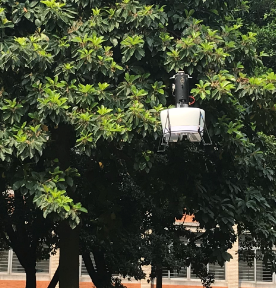
\includegraphics[scale=1]{Fig/DFUAV_f31.png} 
        % 添加标签one_DFUAV以及图标题“涵道风扇式无人机”,标题编号是自动生成的
        \FigureBicaption{\label{one_DFUAV_2}涵道风扇式无人机}{The English caption} 
    \end{figure}
\end{lstlisting}
\begin{figure}[htbp]
    % 图片居中(列居中对齐)
    \centering	
    % 包含当前路径下的Fig文件夹的图片文件DFUAV_f31.png
    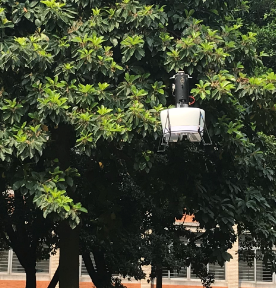
\includegraphics[scale=1]{Fig/DFUAV_f31.png} 
    % 添加标签one_DFUAV以及图标题“涵道风扇式无人机”,标题编号是自动生成的
    \FigureBicaption{\label{one_DFUAV_2}涵道风扇式无人机}{The English caption} 
\end{figure}

值得说明的是,本人修改了cls模版中题注与表格、图片的距离。华工官方提供的格式说明中并未提及中英文题注的行距要求,本人根据上交与清华的博士学位论文格式规范,与几位老师沟通后,修改了题注的行距,具体表现为:
\begin{enumerate}
    \item 中英文题注间保持正文行距,即1.5倍行距。
    \item 中文题注段前\qty{4}{\pt},图片环境下,段后\qty{-8}{\pt};表格环境下,段后\qty{0}{\pt}。
    \item 单独的中或英题注,当文字过长时,应为单倍行距,此处改动暂未实现。(Todo)
\end{enumerate}

若要改动中英文题注间距,可在cls模版对应命令处更改,如下。
\begin{lstlisting}
\newcommand{\FigureBicaption}[2]{
  \renewcommand{\figurename}{图}
  \vspace{4pt} %段前
  \caption{#1}
  \addtocounter{figure}{-1}
  \renewcommand{\figurename}{Fig.}
  \captionsetup{list=false}
  %\vspace{3pt} %中文与英文题注间行距,此行注释掉即保持与正文一致的1.5倍行距。
  \caption{#2}
  \captionsetup{list=true}
  \renewcommand{\figurename}{图}
  \vspace{-8pt} %英文题注段后间距,因float环境默认了一定的间距,经多次尝试后定为-8pt较为美观
}
\end{lstlisting}
\begin{lstlisting}
\newcommand{\TableBicaption}[2]{
  \renewcommand{\tablename}{表}
  \vspace{4pt} %段前
  \caption{#1}
  %\vspace{3pt} %中文与英文题注间行距,此行注释掉即保持与正文一致的1.5倍行距。
  \addtocounter{table}{-1}
  \renewcommand{\tablename}{Table}
  \captionsetup{list=false}
  \caption{#2}
  \captionsetup{list=true}
  \renewcommand{\tablename}{表}
  %\vspace{-2pt} %英文题注段后间距,因表格题注后紧跟表格内容,经试验,此行注释掉较为美观
}
\end{lstlisting}

值得说明的是,原模版对于题注的字号设置为\qty{10.95}{\pt},然而,五号字体应改为\qty{10.5}{\pt},原设置会让题注字号较大。

原模版英文题注比较长时,第二行的题注不再居中,为此,本人修改了figure与table的caption设置,如下:
\begin{lstlisting}
    \captionsetup[figure]{position=bottom,justification=centering}
    \captionsetup[table]{position=top,justification=centering}
\end{lstlisting}
\subsection{超宽图片处理}
有时,个别图片会超出文本区域范围,在原模版文件中,超宽图片左侧边栏默认与文本区域左侧进行左对齐,因此,图片会不在居中位置。为解决这个问题,在图片浮动体命令中,使用下述命令替换\textbackslash{}centering。
\begin{lstlisting}
\setlength{\leftskip}{0pt plus 1fil minus \marginparwidth}
\setlength{\rightskip}{\leftskip}
\end{lstlisting}
\subsection{超宽三线表处理}
有时,三线表结构比较简单,如表\ref{tab:chapter6_featureNumber}所示,表头只有序号与特征,若竖排,会占据非常多的空间,将其转换到横排,需要按照
《CY/T 170—2019学术出版规范表格》,使用双竖细线分隔重复的表头。
\begin{table}[htb]
    \setlength{\belowrulesep}{0pt}
    \setlength{\aboverulesep}{0pt}
    \setlength\arrayrulewidth{0.6pt}
    \centering
    \TableBicaption{特征编号}{The feature number}\label{tab:chapter6_featureNumber}
    \wuhao
    \begin{tabular}{cc||cc||cc}
    \toprule
    序号    &   特征    &   序号    &   特征    &   序号    &   特征\\
    \hhline{--||--||--}
    1   &   $D_1$   &    8    &   $f_5$      &   15    &  $MFCC 6$     \\
    2   &   $R_1$   &    9    &   $E$        &   16    &  $MFCC 7$     \\
    3   &   $K_1$   &    10   &   $MFCC 1$   &   17    &  $MFCC 8$     \\
    4   &   $R_2$   &    11   &   $MFCC 2$   &   18    &  $MFCC 9$     \\
    5   &   $K_2$   &    12   &   $MFCC 3$   &   19    &  $MFCC 10$     \\
    6   &   $f_2$   &    13   &   $MFCC 4$   &   -     &    -   \\
    7   &   $f_4$   &    14   &   $MFCC 5$   &   -     &    -   \\
    \bottomrule
    \end{tabular}
\end{table}

基于这个目的,在导言区外加了makecell与hhline宏包,进行表格的设置,表\ref{tab:chapter6_featureNumber}代码如下:
\begin{lstlisting}
    \begin{table}[htb]
        \setlength{\belowrulesep}{0pt}
        \setlength{\aboverulesep}{0pt}
        \setlength\arrayrulewidth{0.6pt}
        \centering
        \TableBicaption{特征编号}{The feature number}\label{tab:chapter6_featureNumber}
        \wuhao
        \begin{tabular}{cc||cc||cc}
        \toprule
        序号    &   特征    &   序号    &   特征    &   序号    &   特征\\
        \hhline{--||--||--}
        1   &   $D_1$   &    8    &   $f_5$      &   15    &  $MFCC 6$     \\
        2   &   $R_1$   &    9    &   $E$        &   16    &  $MFCC 7$     \\
        3   &   $K_1$   &    10   &   $MFCC 1$   &   17    &  $MFCC 8$     \\
        4   &   $R_2$   &    11   &   $MFCC 2$   &   18    &  $MFCC 9$     \\
        5   &   $K_2$   &    12   &   $MFCC 3$   &   19    &  $MFCC 10$     \\
        6   &   $f_2$   &    13   &   $MFCC 4$   &   -     &    -   \\
        7   &   $f_4$   &    14   &   $MFCC 5$   &   -     &    -   \\
        \bottomrule
        \end{tabular}
    \end{table}
\end{lstlisting}

\section{公式及物理量}
在华工的学位论文要求中,明确了公式及物理量等部分应使用Times New Roman字体,尽管\LaTeX{}默认的字体更为美观。因此,本人修改了cls模版中公式字体设置,并使用siuntix宏包进行物理量的输入。
\subsection{公式环境字体}
尽管原模版中使用了如下代码,但公式及siuntix宏包涉及的物理量仍为默认字体,因此,需要对cls模版进行更改以满足格式要求。
\begin{lstlisting}
    \setmainfont[Mapping=tex-text]{Times New Roman}%\rmfamily 使用的字体,默认英文和数字的字体。
\end{lstlisting}

本文使用mathastext与mathspec宏包更改公式环境字体,在cls模版中,代码如下,注意amsmath宏包一定要在fontspec宏包前声明,fontspec宏包需有no-math的option,最后声明mathspec。
\begin{lstlisting}
    %% 为了实现公式字体为Times New Roman
    \RequirePackage{amsmath}
    \RequirePackage[no-math]{fontspec}
    \RequirePackage{mathspec}
\end{lstlisting}
在正文中,代码如下,需注意,italic选项意在指定公式环境为斜体的Times New Roman。
\begin{lstlisting}
    \usepackage[italic,defaultmathsizes]{mathastext}
\end{lstlisting}
\subsection{物理量}
物理量的格式有两个要求,分别是:
\begin{enumerate}
    \item 物理量本身字体应为Times New Roman。
    \item 物理量中,数字与单位之间应间隔$1/6m$的间距。
\end{enumerate}

本文使用siuntix宏包进行物理量输入,在正文中代码为:
\begin{lstlisting}
\usepackage{siunitx}
\sisetup{input-digits = 0123456789\pi}
\sisetup{per-mode = symbol}%
\DeclareSIUnit \vHardness {Hv} % 维氏硬度Hv
\DeclareSIUnit \dBA {dBA} % 动态范围
\DeclareSIUnit \mT {mT} % 特斯拉
\DeclareSIUnit \pt {pt} % pt
\newcommand{\qtyRange}[3]{\qtyrange[range-units=single,range-phrase=-]{#1}{#2}{#3}} % 单位范围
\newcommand{\numRange}[2]{\numrange[range-phrase=-]{#1}{#2}}	% 数字范围
\end{lstlisting}

本文自定义了输入数字或单位范围的命令,如数字范围命令为\textbackslash{}numRange\{\}\{\},例:\numRange{1}{10};单位范围命令为\textbackslash{}qtyRange\{\}\{\},例:\qtyRange{1}{10}{\mT}。更多
细节请查阅siuntix宏包官方文档。

\section{参考文献}
参考文献相关的修改主要有三个方面,一是连续两篇文献引用时的标注,二是参考文献列表的条目间行距,三是参考文献页末空白的修改。
\subsection{参考文献标注}
对于连续3个以上的参考文献,毫无疑问要标注为[1-3],然而,对于连续2个参考文献,目前大多数老师倾向于标注为[1,2],即\cite{_,_a}。尽管在最新的国标中,连续2个参考文献应标注为[1-2],但本人还是按照老师们的意见,修改了
gb7714-2015宏包对应的代码,使用[1,2]标注格式。相应文件为gb7714-2015.cbx,修改处如下,注意,cbx文件中有多个需要修改的地方,但都有“1改为0”的标注,全局搜索修改即可。
\begin{lstlisting}
%将连续3篇文献压缩改为连续2篇文献压缩
%
%该宏的目的是抛弃压缩内部的编号,而仅输出最后一个编号,主要通过cbx@tempcnta来控制
%一般情况下cbx@tempcnta为0,所以该宏不输出任何内容。当cbx@tempcnta在cite:comp:comp宏中更改变大后
%说明开始进入需要压缩的范围,当到压缩终点时,cbx@tempcnta必然大于1,则输出内容。
%修改第二行的数字1为0即可将默认的3个开始压缩变为2个开始压缩。
\renewbibmacro*{cite:dump}{%
  \ifnumgreater{\value{cbx@tempcnta}}{0}%
    {\ifnumgreater{\value{cbx@tempcnta}}{1}%1改为0,可以将压缩起始3个编号改为2个编号
       {\bibrangedash}%
       {\multicitedelim}%
     \bibhyperref[\cbx@lastkey]{%
       \ifdef\cbx@lastprefix%
         {\printtext[labelprefix]{\cbx@lastprefix}}%
         {}%
       \printtext[labelnumber]{\cbx@lastnumber}}}%
    {}%
  \setcounter{cbx@tempcnta}{0}%
  \global\undef\cbx@lastprefix}
\end{lstlisting}

值得说明的是,gb7714-2015宏包是随着TeXLive安装到电脑上的,最新版已默认标注格式为[1-2],若需要改为[1,2]则按上文说明进行更改,否则无需理会本节内容。
\subsection{参考文献列表条目行距}
原模版的参考文献列表中,条目间行距明显不是1.5倍行距。因此,在主文件中添加了下述语句,保证行距的一致性。
\begin{lstlisting}
\setlength{\bibitemsep}{0ex} % 设置参考文献条目间距离 revised by CYX
\end{lstlisting}
\subsection{参考文献跨页设置}
原始模版中,参考文献存在跨页的默认设置,导致页末(页尾上方)有时存在较大空行,因此,对参考文献进一步设置,取消了排版过大空行。
\begin{lstlisting}
    \renewcommand{\bibsetup}{
        \interlinepenalty=1000\relax
        \widowpenalty=1000\relax
        \clubpenalty=1000\relax
        \raggedbottom
    } % 参考文献条目跨页设置,避免太大空行 by CYX
\end{lstlisting}

\section{标题}
\subsection{单倍行距}
有时,标题的长度会比较长,一行无法全部写下,这时标题会发生换行,而在原模版文件中,全文默认1.5倍行距,因此,这种过长的标题格式会不符合规范,本模版对其进行了更改。由于笔者论文只涉及到了章节标题与各节一级标题的过长,
因此只修改了章节标题与一级标题的行距问题,若使用者有对其他标题格式修改的需要,只需自行添加\textbackslash{}linespread\{1\}命令。
\begin{lstlisting}
\newcommand{\textchapterfont}{\linespread{1}\centering\heiti\xiaoerhao} % 正文上第X章的字体 % 增添了章节标题单倍行距 ---By CYX
\newcommand{\textsectionfont}{\linespread{1}\heiti\xiaosanhao}            % 正文上X.Y节的字体 % 增添了一级标题单倍行距 ---By CYX
\end{lstlisting}
\subsection{三级标题格式}
三级标题应为小四号黑体,居左,原模版设置错误,笔者对其进行了修改。

\section{提交图书馆版}
提交图书馆时,需要末页附上答辩决议,版权页也需要签名,版权页更改可以在word中,对于答辩决议页,在tex文件中增添了下句:
\begin{lstlisting}
    \includepdf[pages=-]{decision.pdf} % 提交图书馆时使用 by CYX
\end{lstlisting}

平常这是注释掉的,最后提交时,将答辩决议保存为pdf文件,使用此句可以附在论文末页。
